\paragraph{QuizziPedia::Front-End::ModelViews::MenuBarModelView}

\label{QuizziPedia::Front-End::ModelViews::MenuBarModelView}

\begin{figure}[ht]
	\centering
	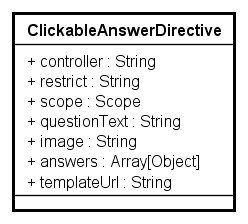
\includegraphics[scale=0.5,keepaspectratio]{UML/Classi/Front-End/QuizziPedia_Front-end_Templates_ClickableAnswerTemplate.png}
	\caption{QuizziPedia::Front-End::ModelViews::MenuBarModelView}
\end{figure} \FloatBarrier

\begin{itemize}
	\item \textbf{Descrizione}: classe di tipo modelview la cui istanziazione è contenuta all'interno della variabile di ambiente \$scope di \textit{Angular.js\ped{G}}. All'interno di essa sono presenti le variabili e i metodi necessari per il \textit{Two-Way Data-Binding\ped{G}} tra la view \texttt{Index} e il controller \texttt{MenuBarController};
	\item \textbf{Utilizzo}: viene utilizzata per effettuare il \textit{Two-Way Data-Binding\ped{G}} tra la view \texttt{Index} e il controller \texttt{MenuBarController} rendendo disponibili variabili e metodi;
	\item \textbf{Relazioni con altre classi}: 
	\begin{itemize}
		\item \textit{IN} \texttt{Index}: pagina alla base di tutte le view dell'applicazione; 
		\item \textit{IN} \texttt{MenuBarController}: questa classe permette di gestire il menù fisso per ogni pagina;
	\end{itemize}
	\item \textbf{Attributi}: 
	\begin{itemize}
		\item ;
	\end{itemize}
	\item \textbf{Metodi}: 
	\begin{itemize}
		\item \texttt{+} \texttt{logOut(): void} \\
		Metodo che richiama il metodo \texttt{logOut} del service \texttt{AuthService} passandogli lo \texttt{username}. Prima di effettuare questa operazione viene mostrato a video un messaggio di conferma per il proseguo dell'operazione; 
		\item \texttt{+} \texttt{logIn(): void} \\
		Metodo che gestisce l’evento click sul pulsante per effettuare il login. Effettua il redirect alla pagina per effettuare il login; 
		\item \texttt{+} \texttt{signUp(): void} \\
		Metodo che gestisce l’evento click sul pulsante per effettuare la registrazione. Effettua il redirect alla pagina per effettuare la registrazione; 
		\item \texttt{+} \texttt{goToUserPage(): void} \\
		Metodo che gestisce l’evento click sul pulsante di visualizzazione della pagina utente. Effettua il redirect alla pagina di visualizzazione della pagina utente; 
		\item \texttt{+} \texttt{goToUserManagemetPage(): void} \\
		Metodo che gestisce l’evento click sul pulsante di gestione del profilo utente. Effettua il redirect alla pagina di gestione del profilo utente; 
		\item \texttt{+} \texttt{goToQuestionsManagementPage(): void} \\
		Metodo che gestisce l’evento click sul pulsante di gestione delle domande. Effettua il redirect alla pagina di gestione delle domande; 
		\item \texttt{+} \texttt{goToQuizManagementPage(): void} \\
		Metodo che gestisce l’evento click sul pulsante di gestione dei questionari. Effettua il redirect alla pagina di gestione dei questionari; 
	\end{itemize}
\end{itemize}

